\documentclass[12pt] {article}

\usepackage[margin=1in]{geometry} %one inch margins
\renewcommand{\baselinestretch}{2} %double space, safe for fancy headers
\usepackage{pslatex} %Times font
\usepackage{apacite} %apa citation style
\bibliographystyle{apacite}
%\usepackage[pdfborder={0 0 0}]{hyperref}%for hyperlinks without ugly boxes
\usepackage{graphicx} %for figures
\usepackage{enumerate} %for lists
\usepackage{fancyhdr} %header
\pagestyle{fancy}
\usepackage[font={small,sf},format=plain,labelfont=bf,up]{caption}
\usepackage{indentfirst}

\fancyhf{}
\fancyhead[l,lo]{Qiao Zhang \textit{ CSE8317 Project Report}} %left top header
\fancyhead[r,ro]{\thepage} %right top header

\begin{document}
\title{Building a Knowledge Graph from Historical Defect Reports with Orthogonal Defect Classification}
\author{Qiao Zhang}
\date \today
\maketitle

\thispagestyle{empty}

\bigskip
%\tableofcontents
\pagebreak
\setcounter{page}{1}
\section{Introduction}
Defect report is commonly a structured natural language artifact generated during the software reliability engineering process.
A well-structured defect report would be very informative to viewers and very efficient for knowledge acquisition purpose.
The previous experience (or knowledge) of handling a specific type of defect would be critical to the success of the future defect analysis.
However, retrieving knowledge from the historical defect reports could be a painful job especially when the volume of reports is high enough.
Based on the experience of a well-known telecommunication equipment company, the number of their historical defect reports has reached 3 million and the number of newly generated defect reports is about 30 thousand each month.
Without an appropriate approach to standardize, formalize, and organize the historical defect reports, it is basically impossible to retrieve knowledge from the gigantic pool of reports.\par

Ontology, as a formal and explicit specification of a shared conceptualization with a complex semantic web structure, is able to standardize and formalize a domain knowledge or the expert interpretation \cite{christina2016an}.
With orthogonal defect classification (ODC), we can not only classify the defect reports into a few specific types but also fit newly generated defect reports into some pre-determined workflows to improve the engineering efficiency.
Both approaches are able to contribute the the objective of improving the knowledge acquisition tasks in software reliability engineering regarding defect anaylsis. 
It might be more beneficial to have them combined as one mechanism since one plus one can be more than two.
Knowledge Graph (KG), which integrates information from various types of resources into an ontology and also applies a reasoning engine to assist deriving new knowledge \cite{ehrlinger2016towards}, is promising to integrate the ODC results into the ontology to effectively and efficiently achieve certain types of knowledge acquisition tasks.
This project aims at conducting a feasibility study to explore the methodoly to build a KG from historical defect reports with ODC.

\section{Background}
\subsection{Ontology}
By formally defining the relationships among entities, ontology is able to provides the intuition of how to further derive the domain knowledge.
As a concept-level knowledge representative for sharing purpose, the potential benefits of applying ontology includes \cite{christina2016an}:
\begin{itemize}
    \item Provide explicit and consistent views of knowledge and distributed information
    \item Support communication among entire development team 
    \item Enable automated data processing and analysis
    \item Improve search quality by taking advantage of its semantic web structure
\end{itemize}
\shortciteA{iliev2012automated} have investigated using ontologies to automatically predict the defect severity based on designed knowledge.
However, it is already beyond the scope of ontology since the author has already introducted a reasoning engine to derieve new knowledge.  
In other word, the ontology might be insufficient for defect analysis especially for an specific instance-level analysis task. 

\subsection{Knowledge Graph}
Knowledge Graph (KG) research has been concentrated by the state-of-the-art literature in recent years since Google posted a blog entry and described how they use KG to enhance their search engine in 2012\footnote{https://googleblog.blogspot.co.at/2012/05/introducing-knowledge-graph-things-not.html}.
The definition of KG has been various from each other until \shortciteA{ehrlinger2016towards} conducted a literature review to synthesize all definitions.
Based on the literature review results, the KG consists of knowledge base and reasoning engine while the ontology is one specific type of knowledge base.
Thus, the defect severity analysis methodology from \shortciteA{iliev2012automated} is very close to the definition of KG, and it proves the necessity of applying KG to the defect analysis domain. 
However, the KG has larger scope than ontology since it is able to integrate more information from difference resources as an instance-level knowledge representative. 

\subsection{Orthogonal Defect Classification}
Orthogonal defect classification (ODC) has been known to reduce the effort of defect analysis especially for root cause analysis \cite{buglione2006introducing}.
With identified root cause, the classified defects can be put into pre-determined workflows that are carefully designed for processing defect effectively and effciently. 
Most existing defect classification approaches and processes are ad hoc and significantly relied on the experience of historical projects and domain expert knowledge of analysts. 
Once the amount of un-classified defects has been accumulated to a certain amount, it will become impossible to be conducted for the ODC analysis.
\shortciteA{huang2015autoodc} have proposed a learning-based automatic ODC (AutoODC) approaches by casting it as a supervised text classification problem.
In this study, the proposed KG is trying to integrate the ontology which contains syntatic data retrieved from defect reports, with the ODC results which can be either manually evaluated or automatically derieved with AutoODC.  

\section{Methodology}
\subsection{Data Collection}
The defect reports investigated in this research are provided by a large telecommunication equipment company with sensitive data desensitized.
The size of dataset to be observed is 10,000 defect reports and most defect reports are bilingual which increased the difficulty of applying AutoODC.
Since the application of AuotODC is not the concentration of this study, we can assume that the ODC analysis can be successfully conducted while the ODC results used in this study are actually derieved manually.
However, the AutoODC is a critical component to the success of building a KG of defect handling since the actual volumn of historical defect reports of the company is considerablely huge.
Due to the privacy consideration and disclosure policy, it is not possible for us to collect the details of how the company process the defect once it is reported and categorized.
The defect handling process mentioned in this study are mostly interpreted from the "solution" part of defect reports and simulated based on the existing knowledge.

\subsection{Building Knowledge Graph}
According to the definition provided by \shortciteA{ehrlinger2016towards}, the design of KG consists of (1) the generation of ontology and (2) the development of reasoning engine.
\subsubsection{Generate Ontology}
Manually building an ontology is commonly an incremental process.
By observing the existing elements included in defect reports, we are able to find the common attributes of a report and each attribute is a node connected to the artifact node "defect report".
Some attribute nodes can be further extended into a set of sub-nodes if a detailed analysis is necessary or the sub-nodes have relationships with other nodes in the ontology.  
For instance, the description is a node connected to the defect report node while the code snippet in the description can be traced to a specific test case or a class-level file in the repository.
Once the initial ontology is generated, the next step is to expand it by finding the external relationships that links the ontology to other knowledge domain.
In this study, the possible external knowledge domain other than the defect report ontology includes defect analysis, code development, testing, risk management, human resource and so on.  
By continuously expanding the ontology either manually or automatically, the included knowledge will be sufficient to upscale to the KG level by adding a reasoning engine upon it.
\subsubsection{Develope Reasoning Engine}
The reasoning engine is designed and developed based on the objective of designing the KG.
In this study, the objective is to build an KG that is able to standardize and formalize the process of handling a defect report once the ODC result retrieved.
Hence, the 

\section{Results and Discussion}
\subsection{Ontology}
\begin{figure*}[h]
    \centering
    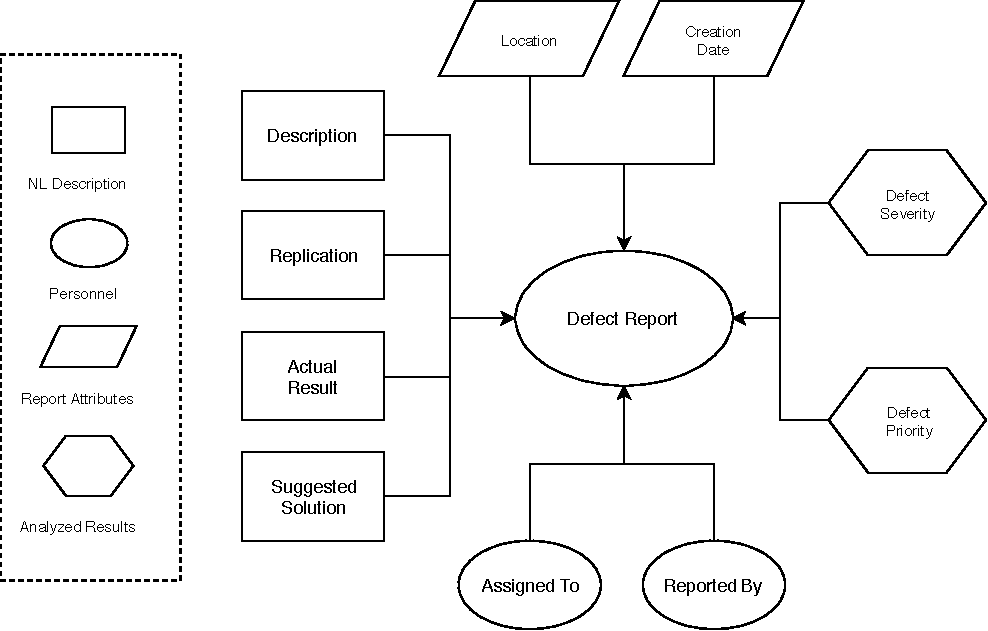
\includegraphics[width=0.8\textwidth]{../figures/OntologyOfDefectReport.pdf}
    \caption{Ontology generated based on defect report}
    \label{fig:defectreport}
\end{figure*}
\subsection{Knowledge Graph}
\subsection{Reasoning Engine}
\subsection{Application Scenario}

\section{Conclusion and Future Works}


\pagebreak
\bibliography{../bib/mybib} %rename to your .bib file
\end{document}
